\documentclass{article}
\usepackage[margin=30mm]{geometry}
\usepackage[comma]{natbib}
\usepackage{todonotes}
\usepackage[toc,page]{appendix}
\usepackage{pdfpages}
\usepackage{graphicx}
\bibliographystyle{agsm}

\begin{document}
\title{Using Facial Recognition to gather Social Media Intelligence}
\author{Jack Neilson}
\maketitle
\newpage
\section{Literature Review}
\subsection{Background}
\subsubsection{SOCMINT}
Social media intelligence (SOCMINT) is an emergent field in intelligence gathering where data is gathered from social media profiles. Massive amounts of data are added to social media services every day \citep{socmintoverview}, much of it personal, making social media sites a potentially valuable resource when gathering information about groups or individuals \citep{gchqmasssurveillance}. Social networks have also been used as a means of communication between persons of interest to the security services, making mining intelligence from their profiles a high priority \citep{socmintoverview}\citep{policesocmint}.

After the 2011 riots in London that were organised in large part on social media, Her Majesty's Inspectorate of Constabulary stated that the police services were "insufficiently equipped" to effectively use SOCMINT in their response \citep{socmintpublicsafety} which suggests that social media intelligence sources may be woefully underutilised \citep{socmintvshumint}. This is not to say that the value of SOCMINT is not realised however, as many intelligence agencies are investing in tools to effectively gather and analyse SOCMINT \citep{socmintpublicsafety} or are performing case studies in to potential uses \citep{bostonbombingcasestudy}.

While traditional human intelligence (HUMINT) focuses on building rapport and a foundation of trust in order to extract information from people of interest \citep{humintinterrogators}, users of social networking websites are much more likely to divulge personal information due to a misplaced senes of privacy \citep{socialmediacontent}. This makes SOCMINT attractive when attempting to gather data with little investment. The amount of data available to gather is vast in comparison to HUMINT sources \citep{socmintoverview}, making mass collection and analysis viable \citep{prismslides}. The nature of SOCMINT makes it easier to analyse than HUMINT, which relies on "tells" and small social cues \citep{humintinterrogators}.

\subsubsection{Uses of SOCMINT}
As previously stated, SOCMINT has seen some emergent use particularly in the security services. The Greek Ministry of Defence has developed a framework to identify individuals fitting certain psychiatric profiles from their social media accounts to allow for early identification of potential insider threats \citep{behaviourdetection}. By identifying factors that multiple intelligence agencies agree make a person more likely to pose an insider threat or negatively influence society (See appendix \ref{appendix:threatgraph}), they were able to map usage habits (intensity, content, popularity) to these factors to draw conclusions about clusters of users. So far, the research has been helpful in insider threat prevention, delinquent behaviour prediction and forensic analysis support.

\subsubsection{Facial Recognition}
Facial recognition is a much more mature area of research than SOCMINT with many examples of industry usage. Facebook uses facial recognition to automate "tagging" photos with the identity of the persons pictured \citep{facebookfacialrecog}, and large companies are now releasing datasets such as YouTube Faces \citep{faceregiondescriptors} in an effort to advance the field.

This is not to say that facial recognition is not without controversy however, as many privacy advocates have pointed out that accurate face regonition could infringe on their right to privacy \citep{gchqmasssurveillance}. David Wood and Lucas Introne have posed that accurate facial recognition could lead to increased levels of surveillance, with no way to "opt out" \citep{facialrecogpolitics}\citep{facialrecogsecurityvsprivacy}.

\subsubsection{Uses of Facial Recognition}
Facial recognition has many practical applications that are already being realised. As noted previously, Facebook uses facial recognition when "tagging" photos. This is presumably done to allow advertisers to more effectively target individual users - for example, a person identified in a photo with a barbeque may receive adverts for propane gas.

Facial recognition is also enjoying a heavy amount of attention from the security services due to it's use in identifying persons of interest. Case studies have been performed using images released to the public to ascertain how effective facial recognition is when looking for a specific person. In particular, Joshua Klontz and Anil Jain performed a case study using the images of the "Boston Bombers" against a set of test data \citep{bostonbombingcasestudy}. Their approach was successful in recognising one of the perpetrators from a picture taken from his social media account (See appendix \ref{appendix:bostonbomber}).

\subsubsection{Constrained vs Unconstrained}
While facial recognition software has come a long way, achieving accuracy rates of up to 99\% on small, consistent data sets \citep{facialrecogidentifyingpoi}, it is still in it's infancy when it comes to identifying people in "unconstrained" images. Images taken in the wild may have large variations in pose, facial occlusion and ambient lighting. This makes it difficult to identify facial features or markers (such as iris distinace, nasal distance, blemishes) which in turn has a negative impact on accuracy rates \citep{unconstrainedfacialrecogbenchmark}. When looking at applications of face recognition software with unconstrained datasets, matches are typically achieved when the test image has similar pose, facial occlusion and lighting as the sample image (See appendix \ref{appendix:bostonbomber}).

\subsection{Theory}
\subsubsection{Prior Work}


\subsection{SOCMINT}
\subsubsection{Prior Knowledge Attacks}


\subsubsection{HUMINT}
Human intelligence (HUMINT) pertains to the gathering of intelligence from individual human subjects. Information may be divulged non-consensually e.g. in the case of interrogation \citep{criminalvshumint}, or consensually in the case of clandestine information gathering \citep{clandestinehumint}. 

Non-consensual information gathering via interview or interrogation has only recently become a subject of study for the general public \citep{humintinterrogators}. 

Consensual information gathering sits in a much more grey area. Presenting yourself as somebody else may not be illegal depending on the circumstances, however it poses several moral questions. Clandestine intelligence gathering is still an extremely effective strategy, particularly when attempting to gather sensitive information which may be more heavily protected e.g. airgapped, firewalled \citep{clandestinehumint}. This makes it attractive during wartime or times of civil unrest \citep{humintni}\citep{humintcyberage}

Using a human intelligence approaches when gathering information has several downsides. It is a high risk strategy, as should a person be found out the consequences can be severe \citep{humintni}. The potential reward of sensitive information may be deemed to not be worth the risk. It goes without saying that HUMINT does not scale particularly well - it is a useful tool when attempting to extract information from a single person or small group, but it is much less useful when gathering information about larger groups. It relies on trust being built and may be ineffective when attempting to gather information from targets trained in tradecraft \citep{humintni}\citep{clandestinehumint}\citep{humintcyberage}.

\subsubsection{Social Engineering}

\subsubsection{Spearphish}

\subsubsection{Individual vs Group Data}

\subsubsection{Quantity of Information}

\subsubsection{Accessibility of Data}

\subsubsection{Uses}
\todo{PRISM}

\subsubsection{Challenges and Constraints}







\subsection{Facial Recognition}
\subsubsection{Current Applications}

\subsubsection{State of the Art}	

\subsubsection{Challenges}

\subsubsection{Recent Advances}

\subsubsection{Unconstrained Facial Recognition}

\subsubsection{Application to Social Media}

\newpage
\bibliography{citations}

\newpage
\begin{appendices}
\section{Threat Graph}
\label{appendix:threatgraph}
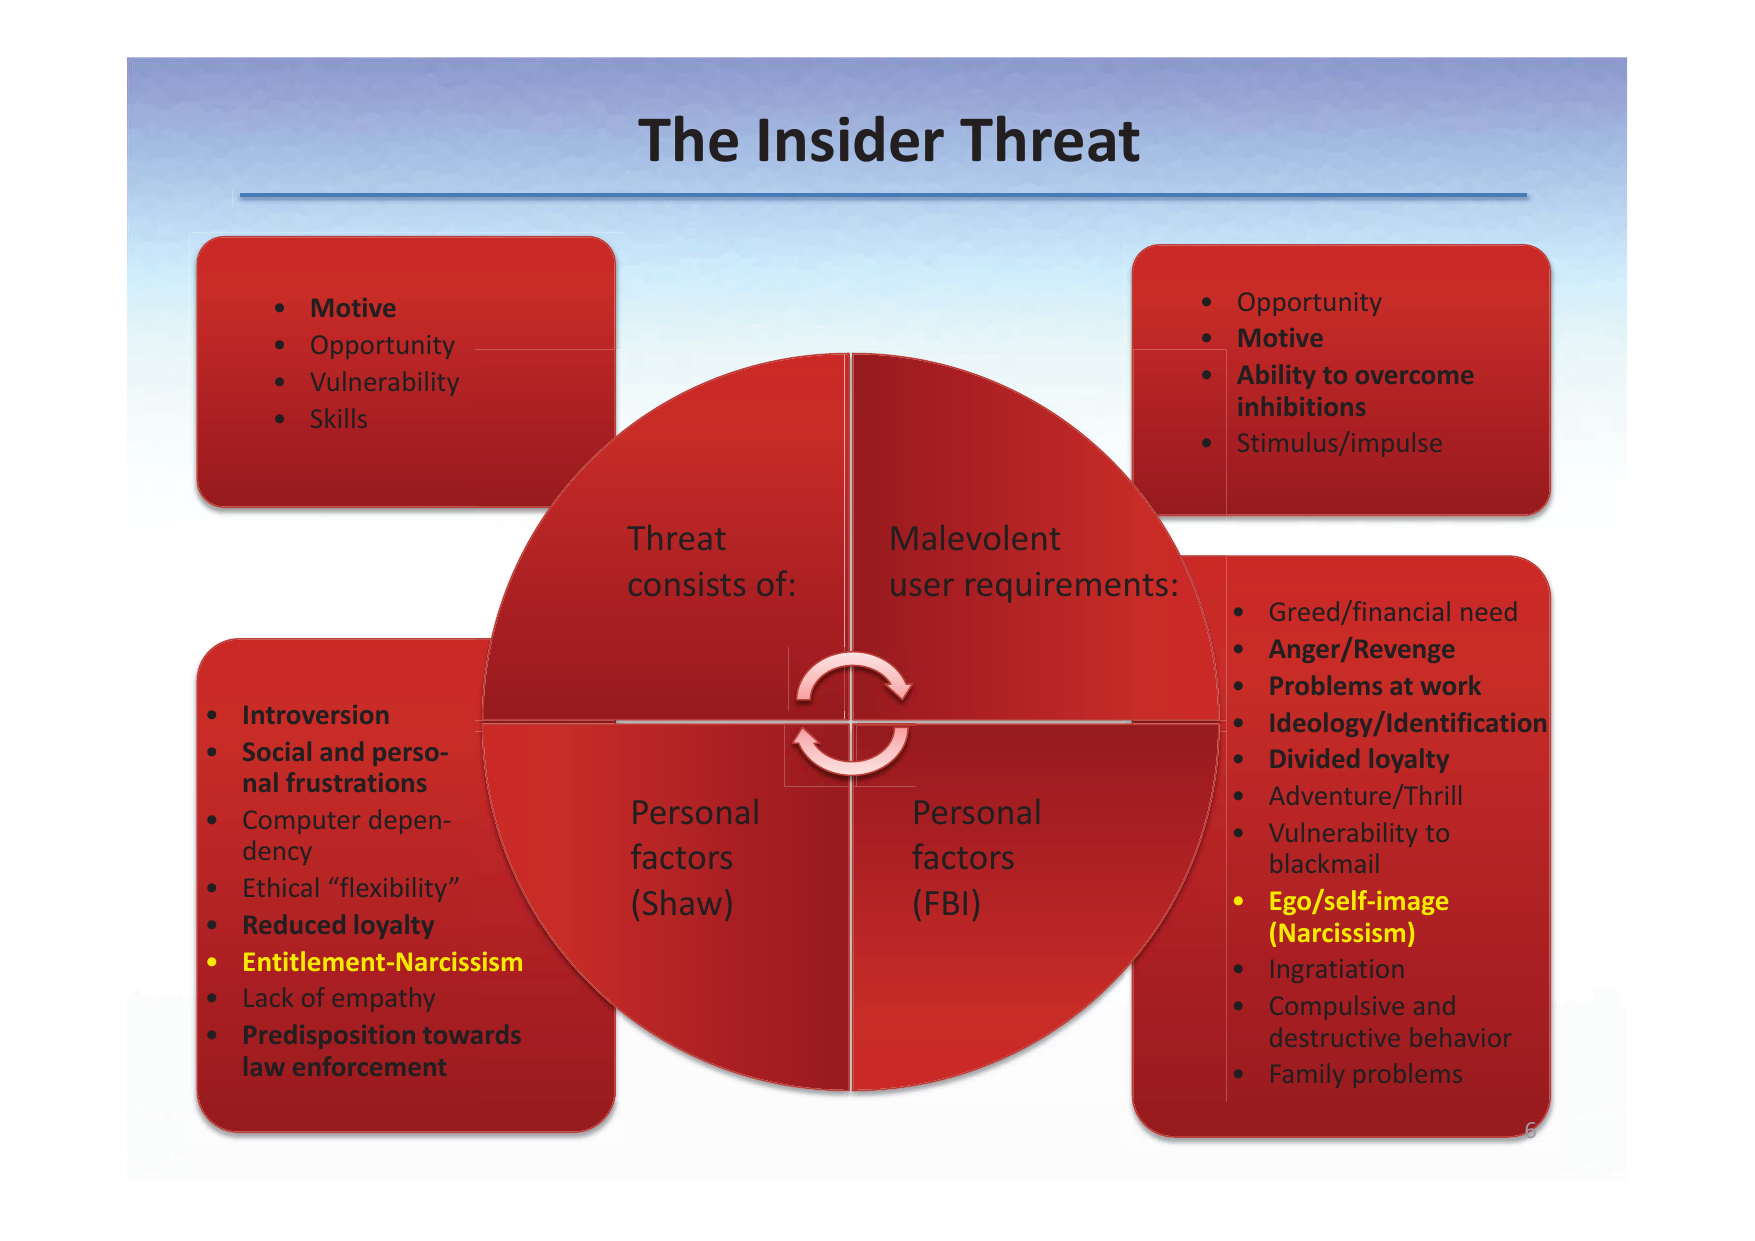
\includegraphics[width=\linewidth]{res/threat_graph.png}
Graph of insider threat factors \citep{behaviourdetection}.

\section{"Boston Bomber" Identification}
\label{appendix:bostonbomber}
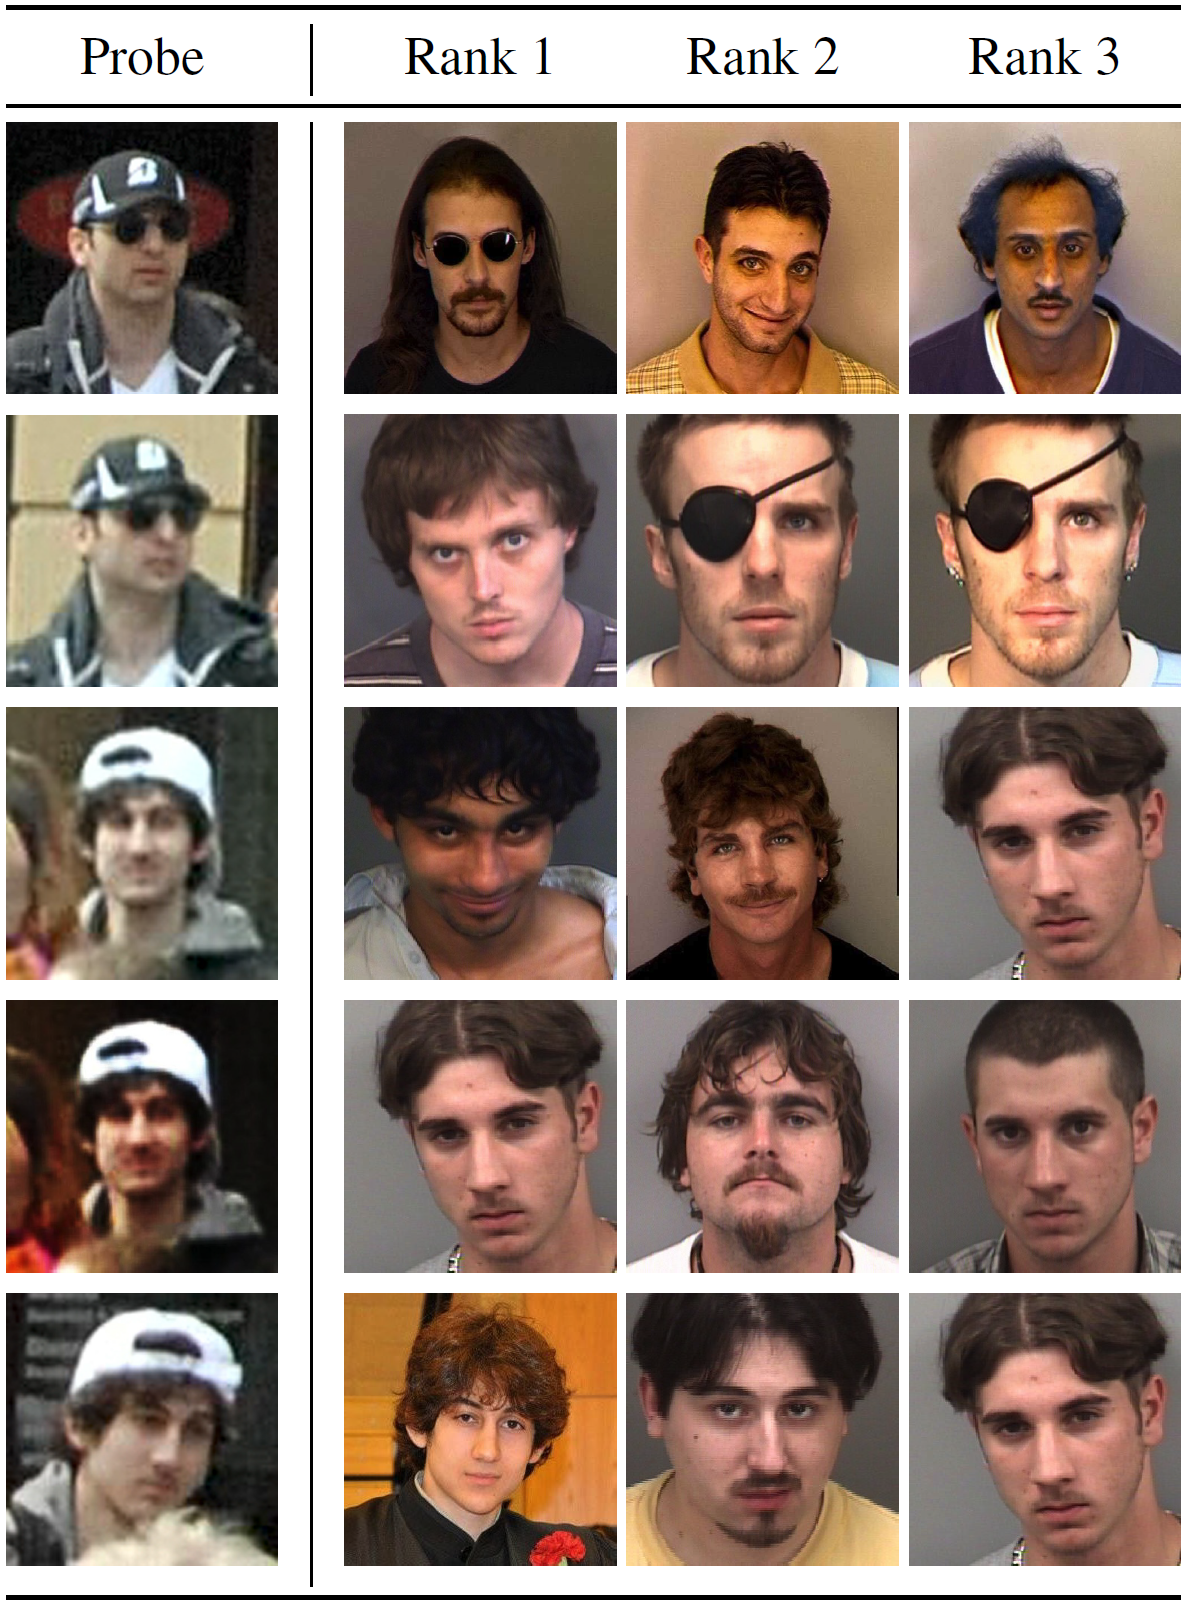
\includegraphics[width=\linewidth]{res/boston_bomber.png}
Table of potential matches, note the correct identification from the picture taken from social media with similar pose and lighting \citep{bostonbombingcasestudy}.

\end{appendices}

\end{document}